\documentclass[10pt,aspectratio=169]{beamer}

\usetheme[numbering=fraction,progressbar=frametitle]{metropolis}
\usefonttheme{professionalfonts}
\usepackage[UTF8]{ctex}
\usepackage{appendixnumberbeamer}
\usepackage{amsmath,amssymb,bm}
\usepackage{booktabs}
\usepackage{graphicx}

\title{Shape Function 生成器}
\subtitle{方法设计、验证样例与当前实验信号}
\author{shape\_function-main}
\date{\today}

\newcommand{\xq}{\mathbf{x}_q}
\newcommand{\Xnode}{\mathbf{X}_i}
\newcommand{\ri}{\mathbf{r}_i}
\newcommand{\rhat}{\hat{\mathbf{r}}_i}
\newcommand{\phii}{\phi_i(\mathbf{x}_q)}
\newcommand{\phiref}{\phi_i^{\mathrm{ref}}(\mathbf{x}_q)}

\begin{document}

\maketitle

\begin{frame}{问题定义}
  \begin{columns}[T,onlytextwidth]
    \column{0.56\textwidth}
      我们在 query-centered patch 上学习一个局部生成器：
      \[
      \mathcal{G}_{\theta}:
      \left(
      \xq,\{\Xnode\}_{i=1}^{k},\beta,\rho_q
      \right)
      \mapsto
      \{\phii\}_{i=1}^{k}
      \]

      \vspace{0.5em}
      \begin{itemize}
        \item 输入：局部节点云、查询点、支撑形状参数、几何上下文
        \item 输出：该局部 patch 上的 shape-function 权值
        \item 目标：得到快速的无网格 warm start，而不是做全局场预测
      \end{itemize}

    \column{0.40\textwidth}
      \begin{block}{结构约束}
        \[
        \sum_i \phi_i = 1,
        \qquad
        \sum_i \phi_i \Xnode = \xq
        \]
      \end{block}

      \begin{alertblock}{数值意义}
        Partition of unity 与一阶一致性是最核心的结构约束。
      \end{alertblock}
  \end{columns}
\end{frame}

\begin{frame}{方法总览}
  \[
  \left(\xq,\{\Xnode\},\beta,\rho_q\right)
  \xrightarrow{\text{feature construction}}
  \{\mathbf{f}_i\}
  \xrightarrow{\text{backbone}}
  \{l_i\}
  \xrightarrow{\text{B1--B4 head}}
  \{\phi_i\}
  \]

  \vspace{0.8em}
  \begin{columns}[T,onlytextwidth]
    \column{0.48\textwidth}
      \begin{block}{Backbone}
        \begin{itemize}
          \item 编码局部几何与 patch 内交互
          \item 从无网格节点集产生原始 logits
          \item 当前主模型为 kernel-operator
        \end{itemize}
      \end{block}

    \column{0.48\textwidth}
      \begin{block}{Structure-preserving head}
        \begin{itemize}
          \item 提供正性偏置与 locality 控制
          \item 做 partition-of-unity 归一化
          \item 通过 reproducing correction 恢复一致性
      \end{itemize}
      \end{block}
  \end{columns}
\end{frame}

\begin{frame}{局部几何编码}
  \begin{columns}[T,onlytextwidth]
    \column{0.58\textwidth}
      \[
      \ri = \Xnode - \xq,
      \qquad
      r_{\max} = \max_i \|\ri\|,
      \qquad
      \rhat = \frac{\ri}{r_{\max}}
      \]

      \[
      \mathbf{f}_i =
      \left[
      \rhat,\;
      \|\rhat\|,\;
      \beta,\;
      \rho_q
      \right]
      \]

      \begin{itemize}
        \item Query-centered normalization 去掉平移歧义
        \item Scale normalization 提高跨 patch 的可比性
        \item $\rho_q$ 汇总 patch 密度、各向异性与局部复杂度
      \end{itemize}

    \column{0.38\textwidth}
      \begin{alertblock}{Support radius 修正}
        Backbone 仍使用 $r_{\max}$ 做归一化尺度，但 head 使用
        \[
        r_{\mathrm{support}} = \alpha r_{\max},
        \qquad \alpha = 1.05
        \]
        这样最远邻居不再被窗口函数系统性压成 0。
      \end{alertblock}
  \end{columns}
\end{frame}

\begin{frame}{Kernel-Operator 主干}
  \begin{columns}[T,onlytextwidth]
    \column{0.60\textwidth}
      \[
      \mathbf{h}_i^{(0)} = \mathrm{MLP}_{\mathrm{lift}}(\mathbf{f}_i)
      \]

      \[
      \mathbf{g}_{ij}^{(\ell)} =
      \left[
      \mathbf{h}_i^{(\ell)}-\mathbf{h}_j^{(\ell)},
      \hat{\mathbf{r}}_i,\hat{\mathbf{r}}_j,
      \|\hat{\mathbf{r}}_i-\hat{\mathbf{r}}_j\|
      \right]
      \]

      \[
      \alpha_{ij}^{(\ell)} =
      \mathrm{softplus}\!\left(\mathrm{MLP}_{\mathrm{mod}}(\mathbf{g}_{ij}^{(\ell)})\right)
      \cdot
      w_{\mathrm{Wendland}}(\|\hat{\mathbf{r}}_i-\hat{\mathbf{r}}_j\|)
      \]

      \[
      \mathbf{h}_i^{(\ell+1)} =
      \mathbf{h}_i^{(\ell)} +
      \sum_j \bar{\alpha}_{ij}^{(\ell)} \mathbf{V}^{(\ell)}\mathbf{h}_j^{(\ell)}
      \]

    \column{0.36\textwidth}
      \begin{block}{设计动机}
        \begin{itemize}
          \item 对节点集合具备 permutation awareness
          \item 依赖相对几何，而不是规则网格结构
          \item 相比 sorted-distance MLP baseline，归纳偏置更合理
        \end{itemize}
      \end{block}
  \end{columns}
\end{frame}

\begin{frame}{Structure-Preserving Head}
  \begin{columns}[T,onlytextwidth]
    \column{0.60\textwidth}
      \textbf{B1 Softplus}
      \[
      \phi_i^{(1)} = \mathrm{softplus}(l_i)
      \]

      \textbf{B2 Window modulation}
      \[
      \phi_i^{(2)} =
      \phi_i^{(1)}
      \cdot
      w\!\left(\frac{\|\ri\|}{r_{\mathrm{support}}}\right)
      \]

      \textbf{B3 Normalization}
      \[
      \phi_i^{\mathrm{base}} =
      \frac{\phi_i^{(2)}}{\sum_j \phi_j^{(2)} + \varepsilon}
      \]

      \textbf{B4 Reproducing correction}
      \[
      \phi_i =
      \phi_i^{\mathrm{base}}
      +
      \phi_i^{\mathrm{base}} \mathbf{p}_i^\top
      \mathbf{M}^{-1}
      \left(
      \mathbf{b} - \sum_j \phi_j^{\mathrm{base}}\mathbf{p}_j
      \right)
      \]

    \column{0.36\textwidth}
      \begin{block}{各阶段作用}
        \begin{itemize}
          \item B1：稳定的正性偏置
          \item B2：locality 与紧支撑
          \item B3：partition of unity
          \item B4：一阶一致性
        \end{itemize}
      \end{block}

      \begin{alertblock}{关键点}
        B4 之后不能再做归一化，否则一致性修正会被破坏。
      \end{alertblock}
  \end{columns}
\end{frame}

\begin{frame}{Teacher 与训练目标}
  \begin{columns}[T,onlytextwidth]
    \column{0.58\textwidth}
      \textbf{Patch-level max-ent teacher}
      \[
      z_i = w_i \exp(-\ri^\top \bm{\lambda}),
      \qquad
      \phiref = \frac{z_i}{\sum_j z_j}
      \]

      Gaussian prior:
      \[
      w_i = \exp\!\left(
      -\beta \left(\frac{\|\ri\|}{r_{\max}}\right)^2
      \right)
      \]

      \vspace{0.4em}
      \textbf{训练损失}
      \[
      \mathcal{L} =
      \mathcal{L}_{\mathrm{data}}
      +
      \lambda_{\mathrm{cons}} \mathcal{L}_{\mathrm{cons}}
      +
      \lambda_{\mathrm{neg}} \mathcal{L}_{\mathrm{neg}}
      \]

      \[
      \mathcal{L}_{\mathrm{cons}} =
      \left(\sum_i \phi_i - 1\right)^2 +
      \left\|
      \sum_i \phi_i \Xnode - \xq
      \right\|^2
      \]

    \column{0.38\textwidth}
      \begin{block}{解释}
        \begin{itemize}
          \item Teacher 提供 reference-guided warm start
          \item Data term 拟合 max-ent 参考解
          \item 约束项与负值惩罚项用于稳定训练
        \end{itemize}
      \end{block}

      \begin{exampleblock}{主要指标}
        \begin{itemize}
          \item relative L2
          \item PoU residual
          \item linear residual
          \item negative fraction
          \item cond($M$)
        \end{itemize}
      \end{exampleblock}
  \end{columns}
\end{frame}

\begin{frame}{首轮生产规模结果}
  \begin{columns}[T,onlytextwidth]
    \column{0.57\textwidth}
      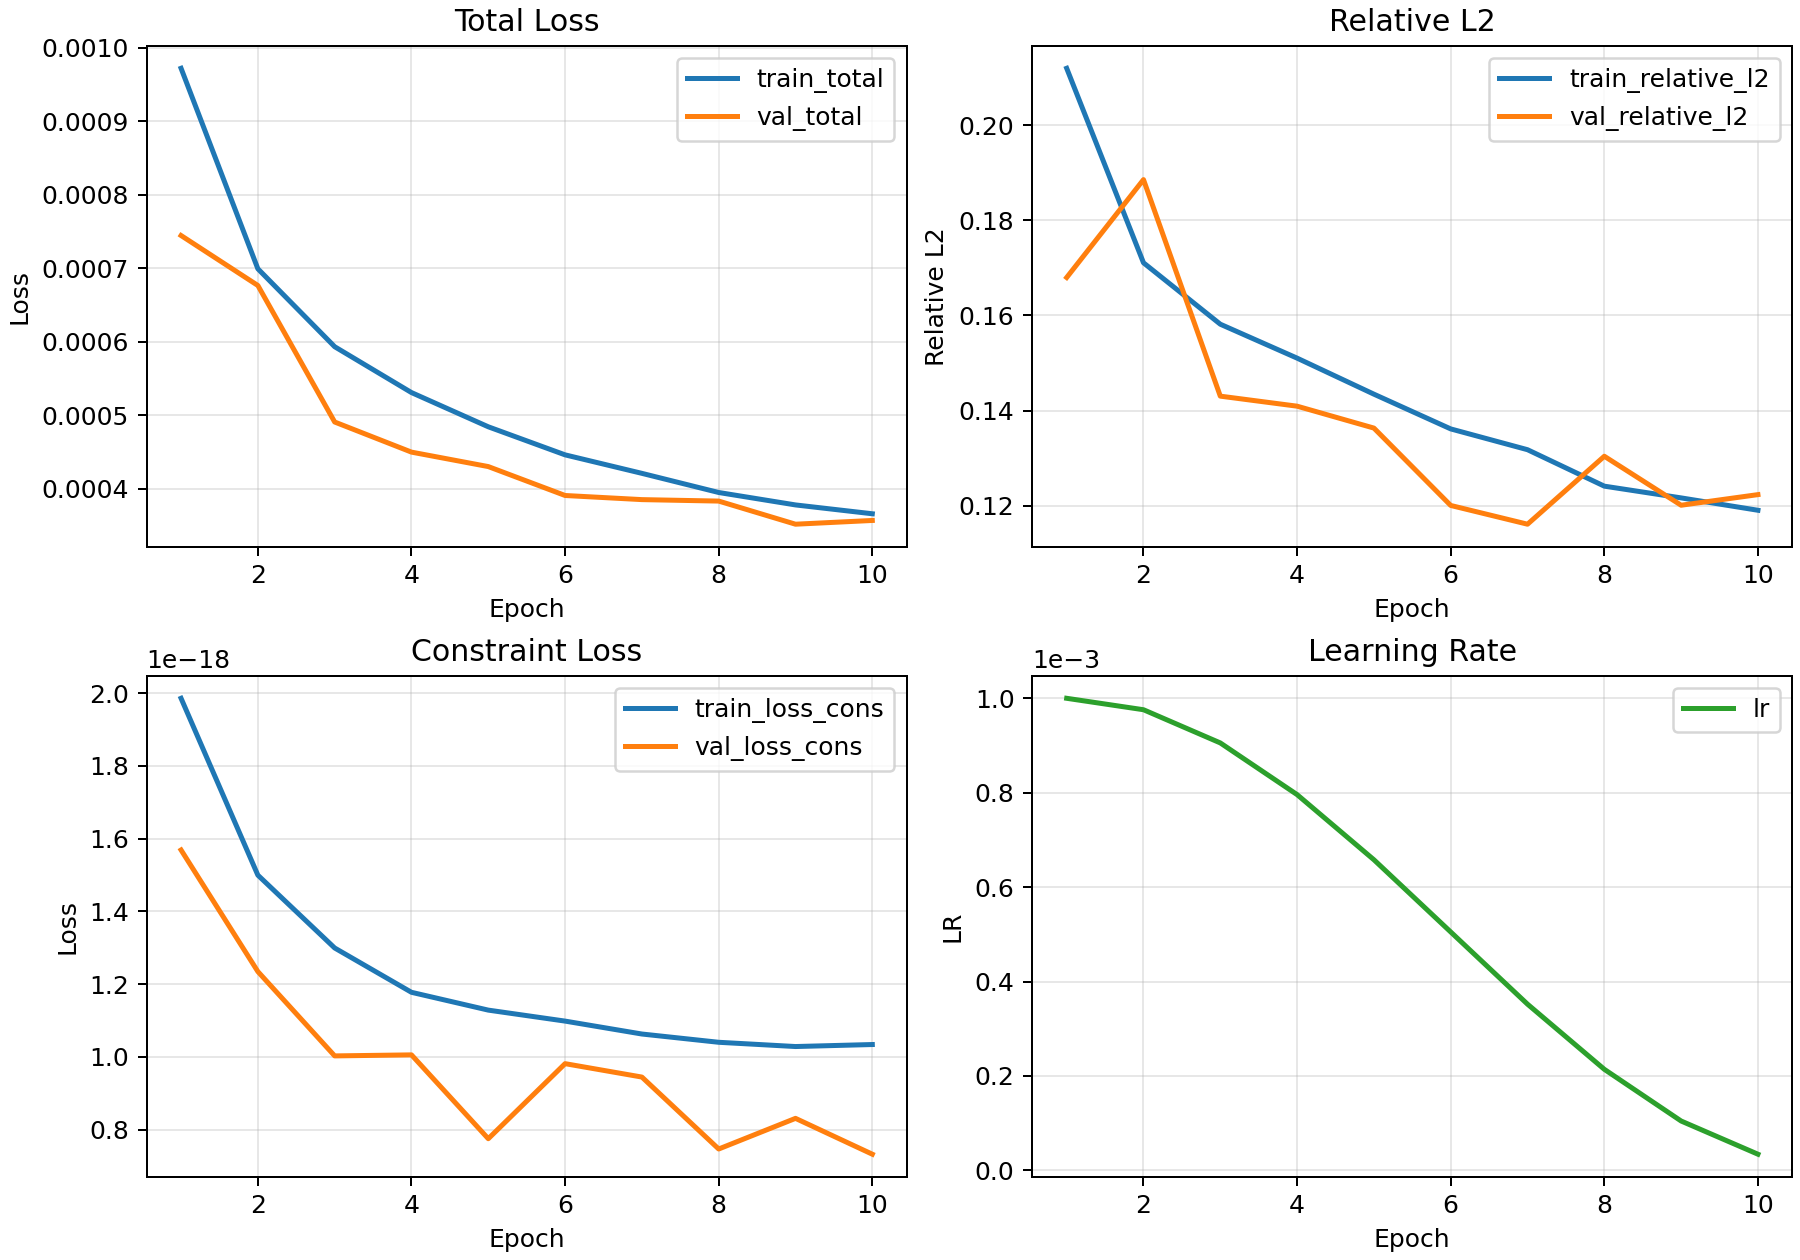
\includegraphics[width=\linewidth]{figures/training_curves_kernel.png}

    \column{0.40\textwidth}
      \begin{table}
        \small
        \begin{tabular}{@{}lcc@{}}
          \toprule
          Metric & Kernel & MLP \\
          \midrule
          relative L2 & 0.1201 & 0.1791 \\
          global $L_\infty$ & 0.1969 & 0.2540 \\
          neg. fraction & 0.0464 & 0.0776 \\
          mean cond($M$) & 646.3 & 584.5 \\
          \bottomrule
        \end{tabular}
      \end{table}

      \vspace{0.6em}
      \begin{alertblock}{初步结论}
        首轮 production run 中，kernel backbone 在主要精度指标上优于 MLP baseline。
      \end{alertblock}
  \end{columns}
\end{frame}

\begin{frame}{对比视图}
  \begin{columns}[T,onlytextwidth]
    \column{0.56\textwidth}
      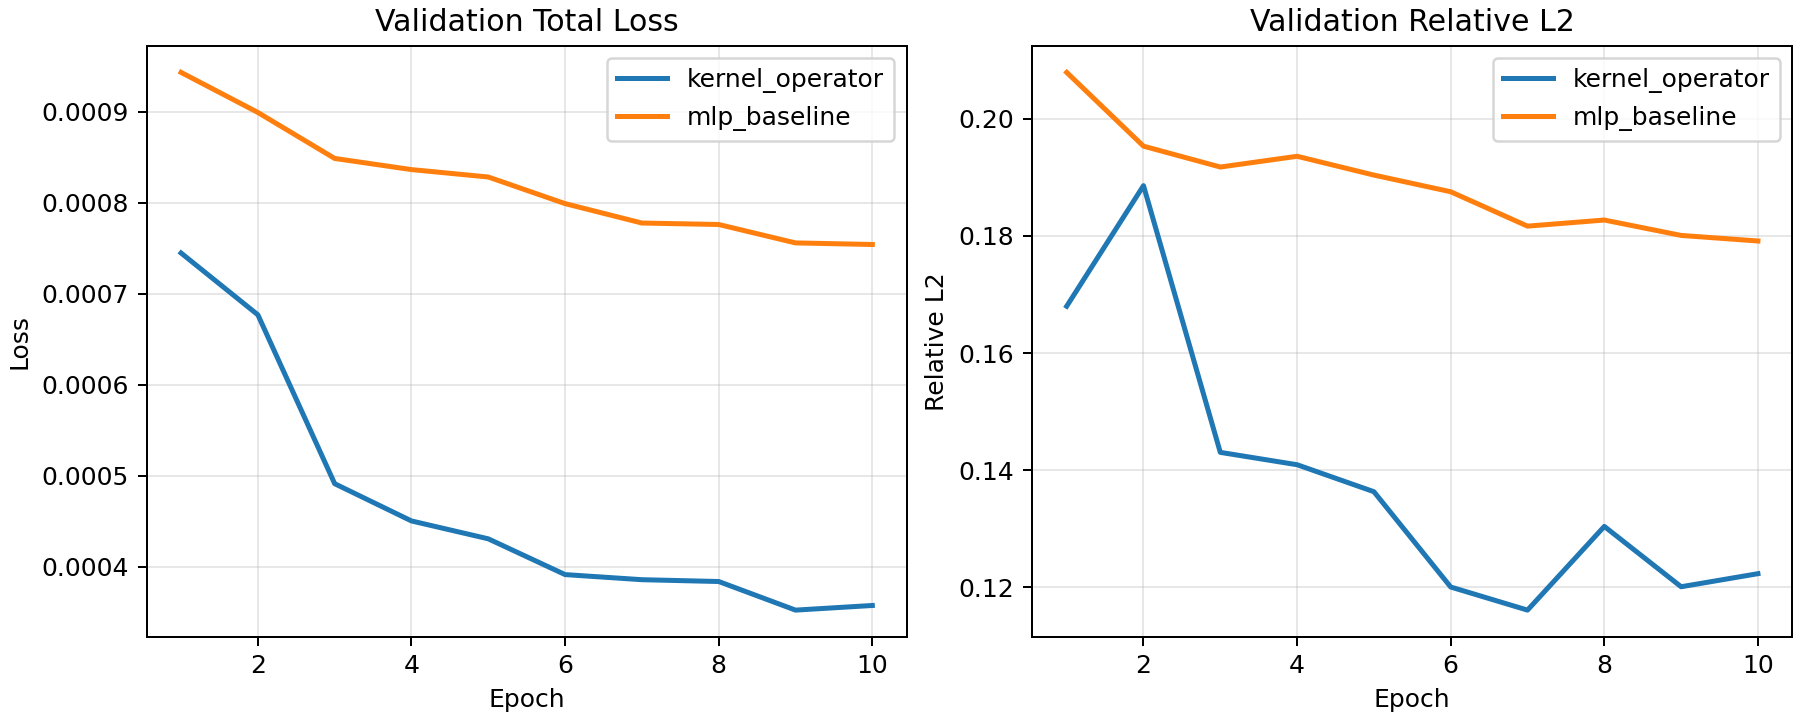
\includegraphics[width=\linewidth]{figures/comparison_kernel_vs_mlp.png}

    \column{0.40\textwidth}
      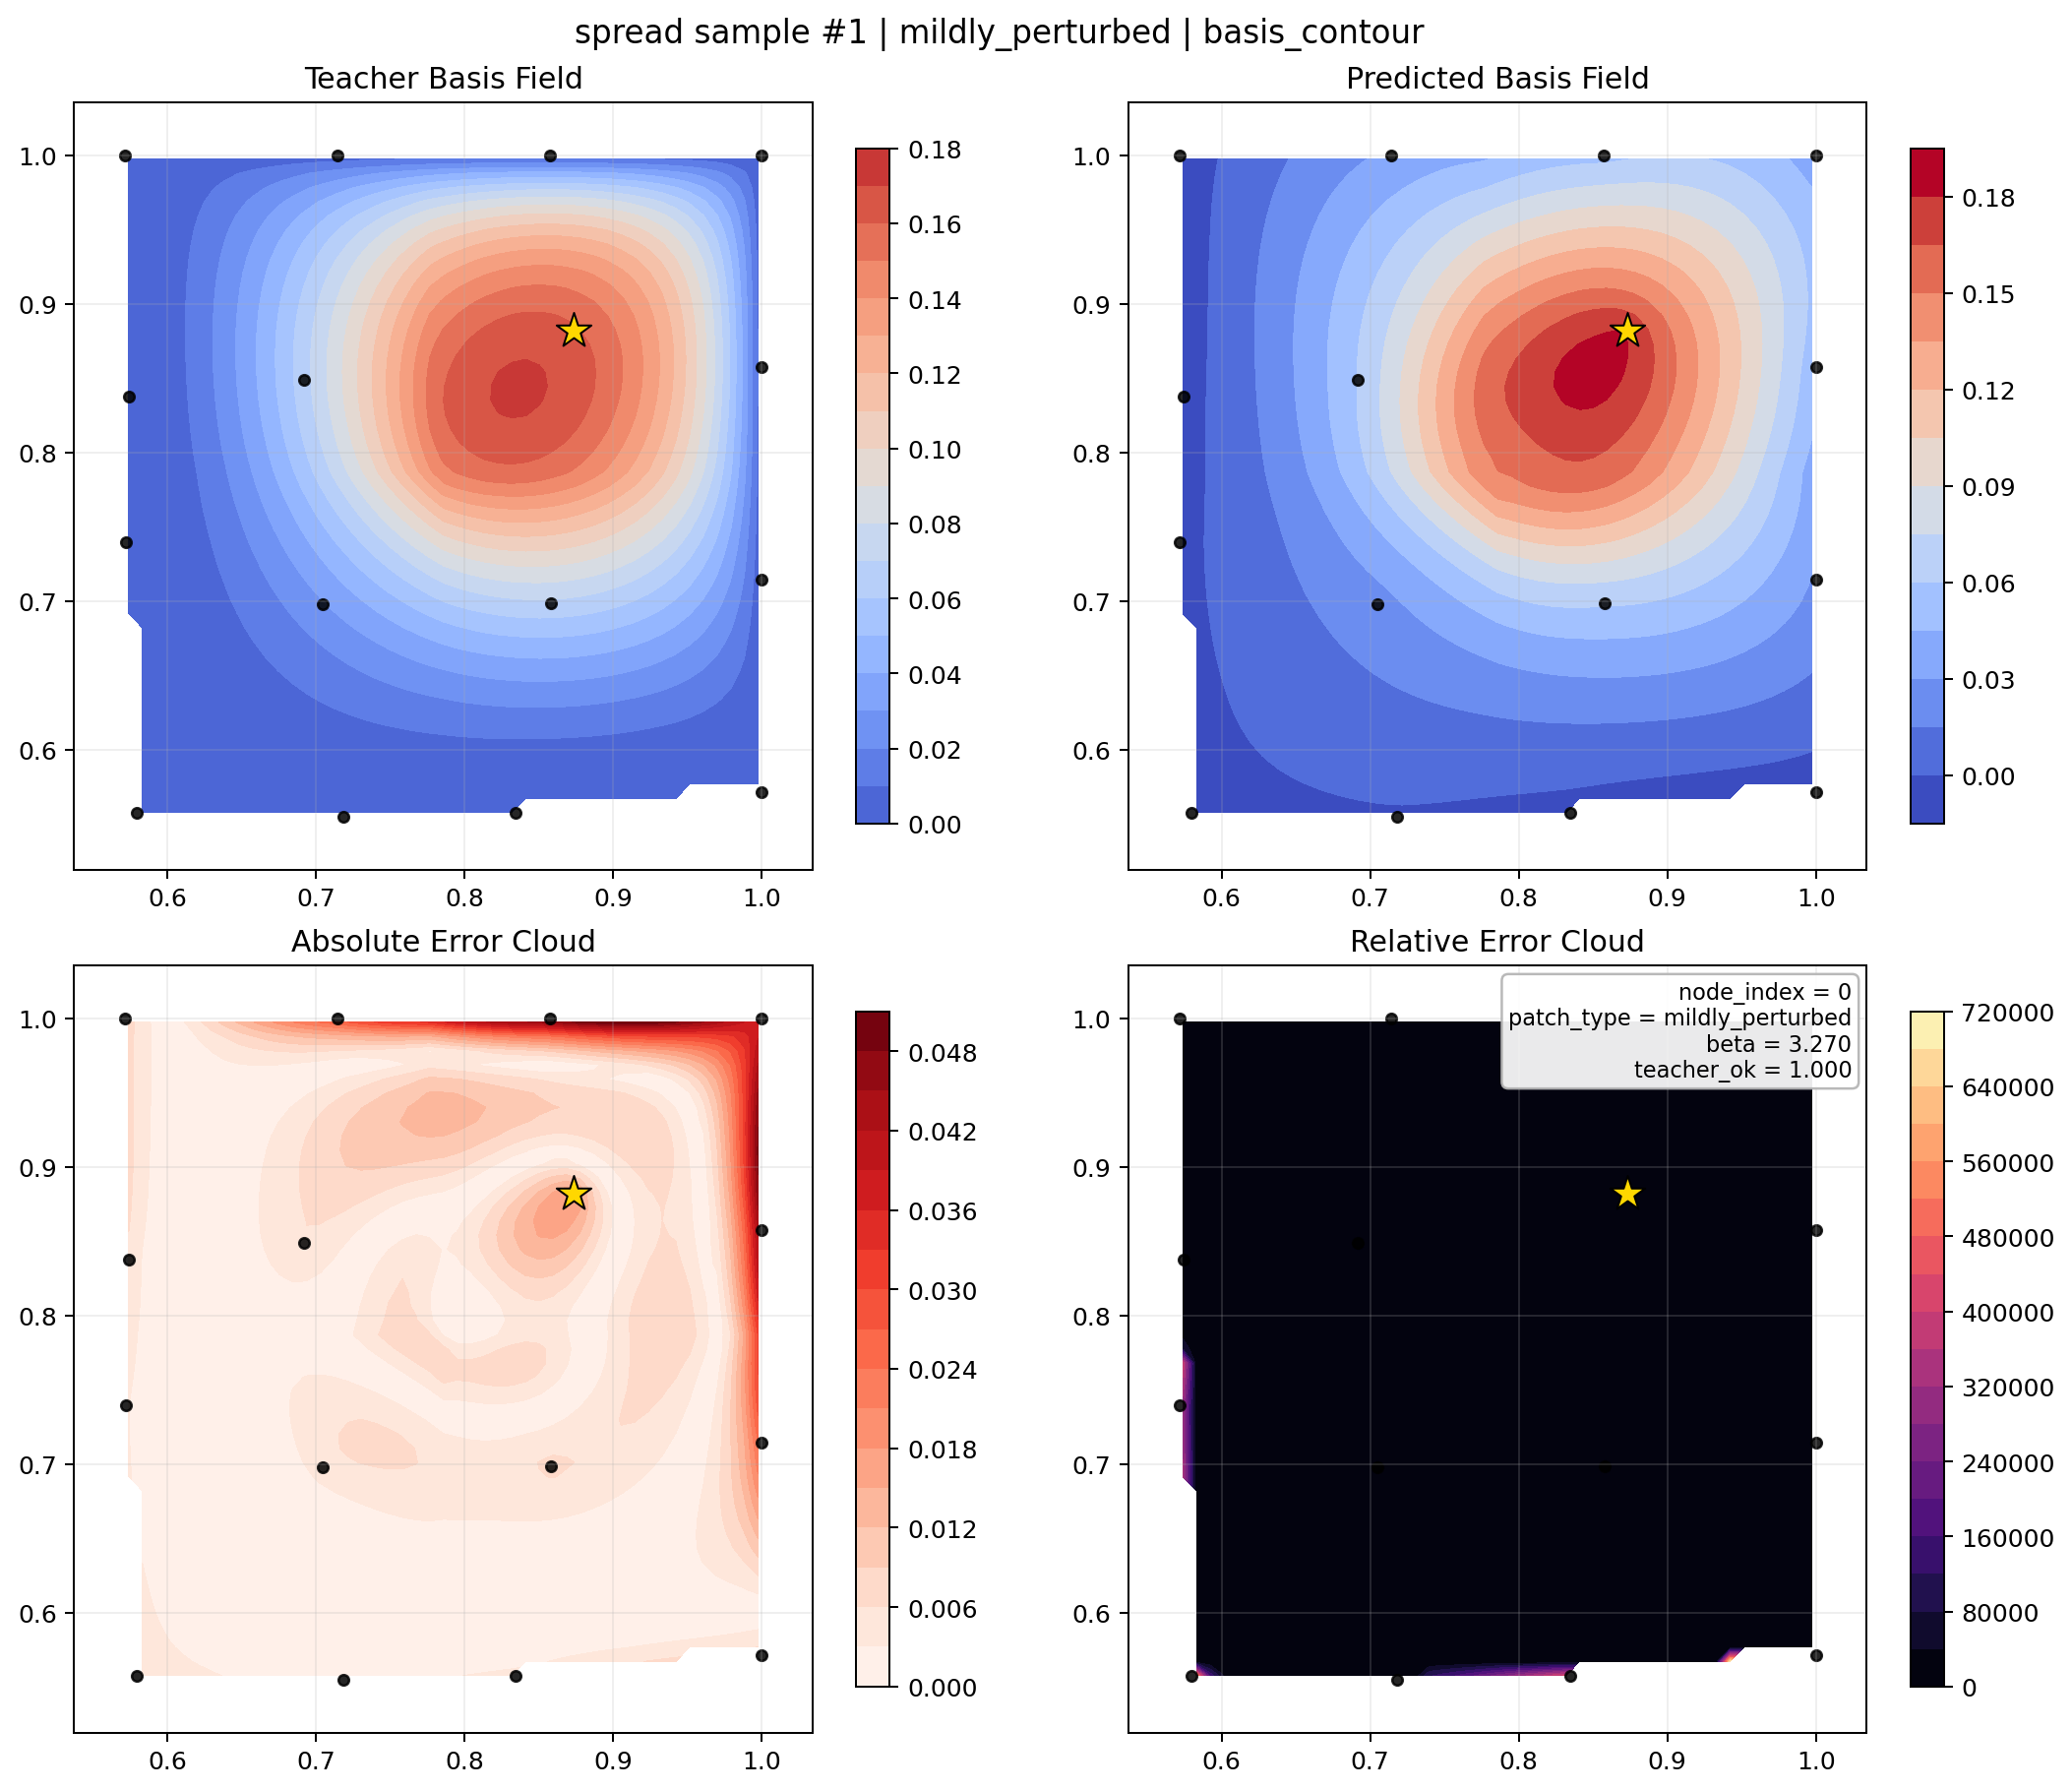
\includegraphics[width=\linewidth]{figures/basis_contour_good.png}

      \vspace{0.5em}
      \small
      左：kernel 与 MLP 的整体对比。\\
      右：一个常规 patch 上的 clean basis contour。
  \end{columns}
\end{frame}

\begin{frame}{常规样例：基函数视图}
  \begin{columns}[T,onlytextwidth]
    \column{0.48\textwidth}
      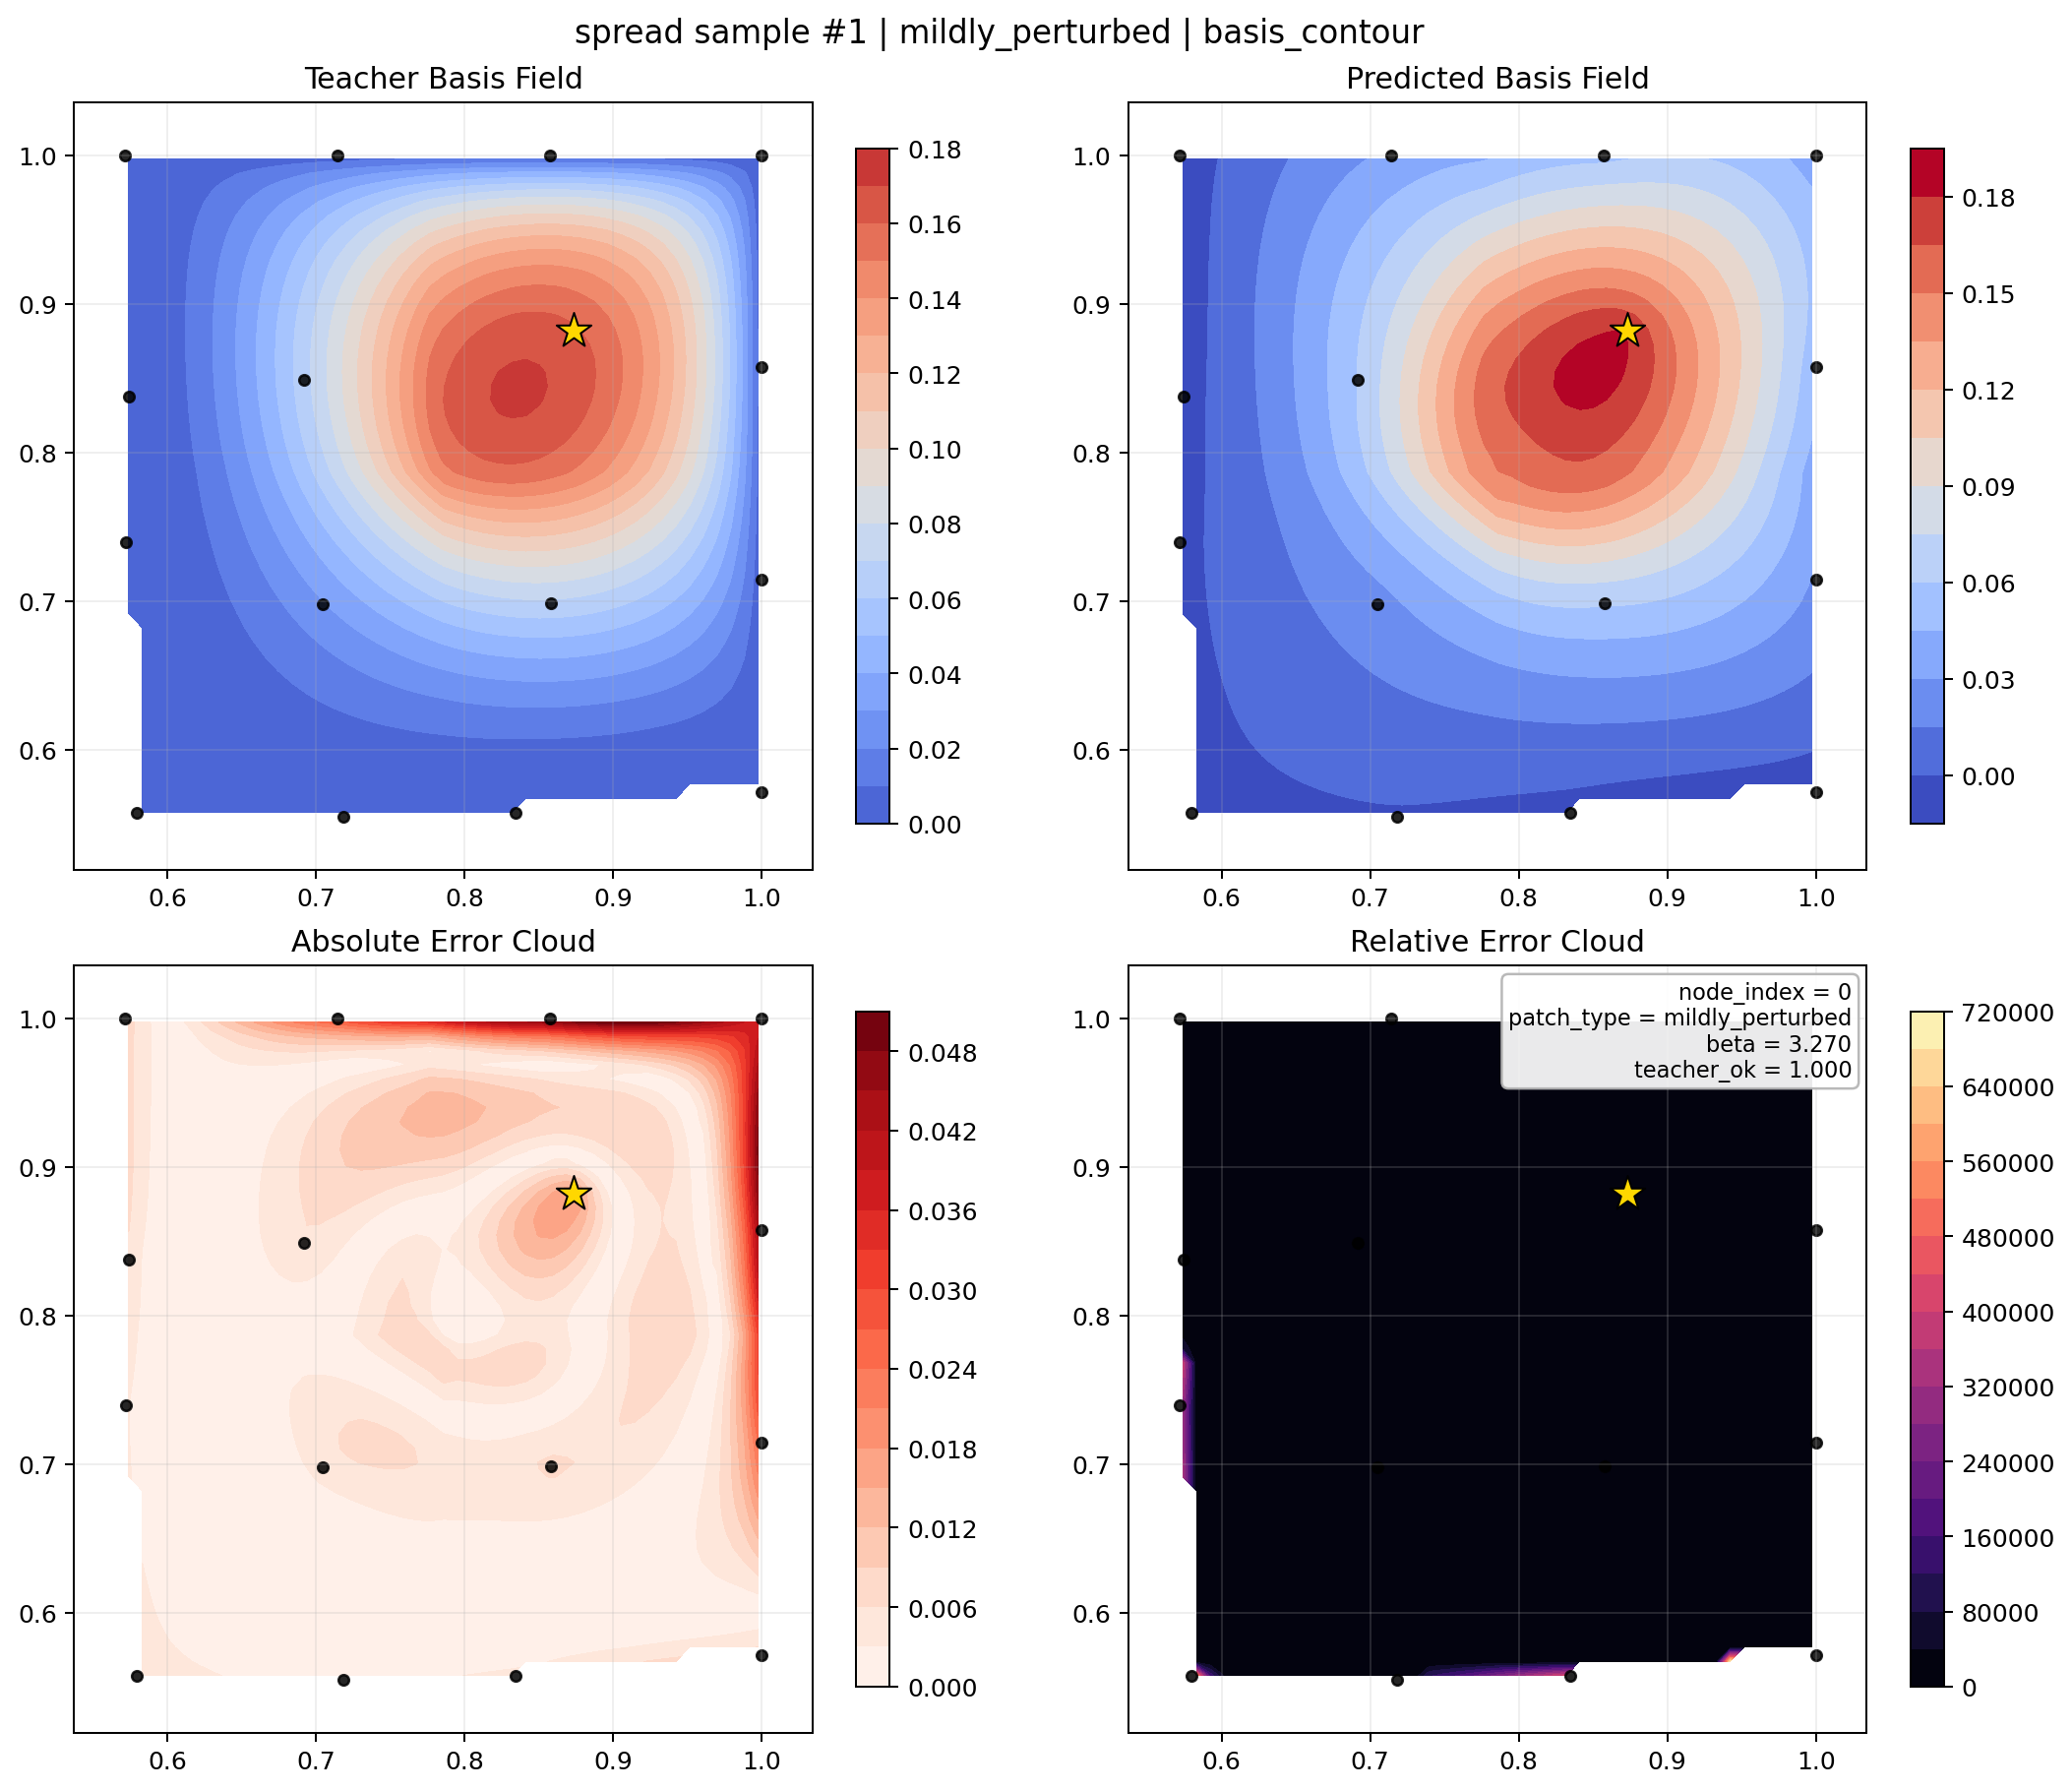
\includegraphics[width=\linewidth]{figures/basis_contour_good.png}

    \column{0.48\textwidth}
      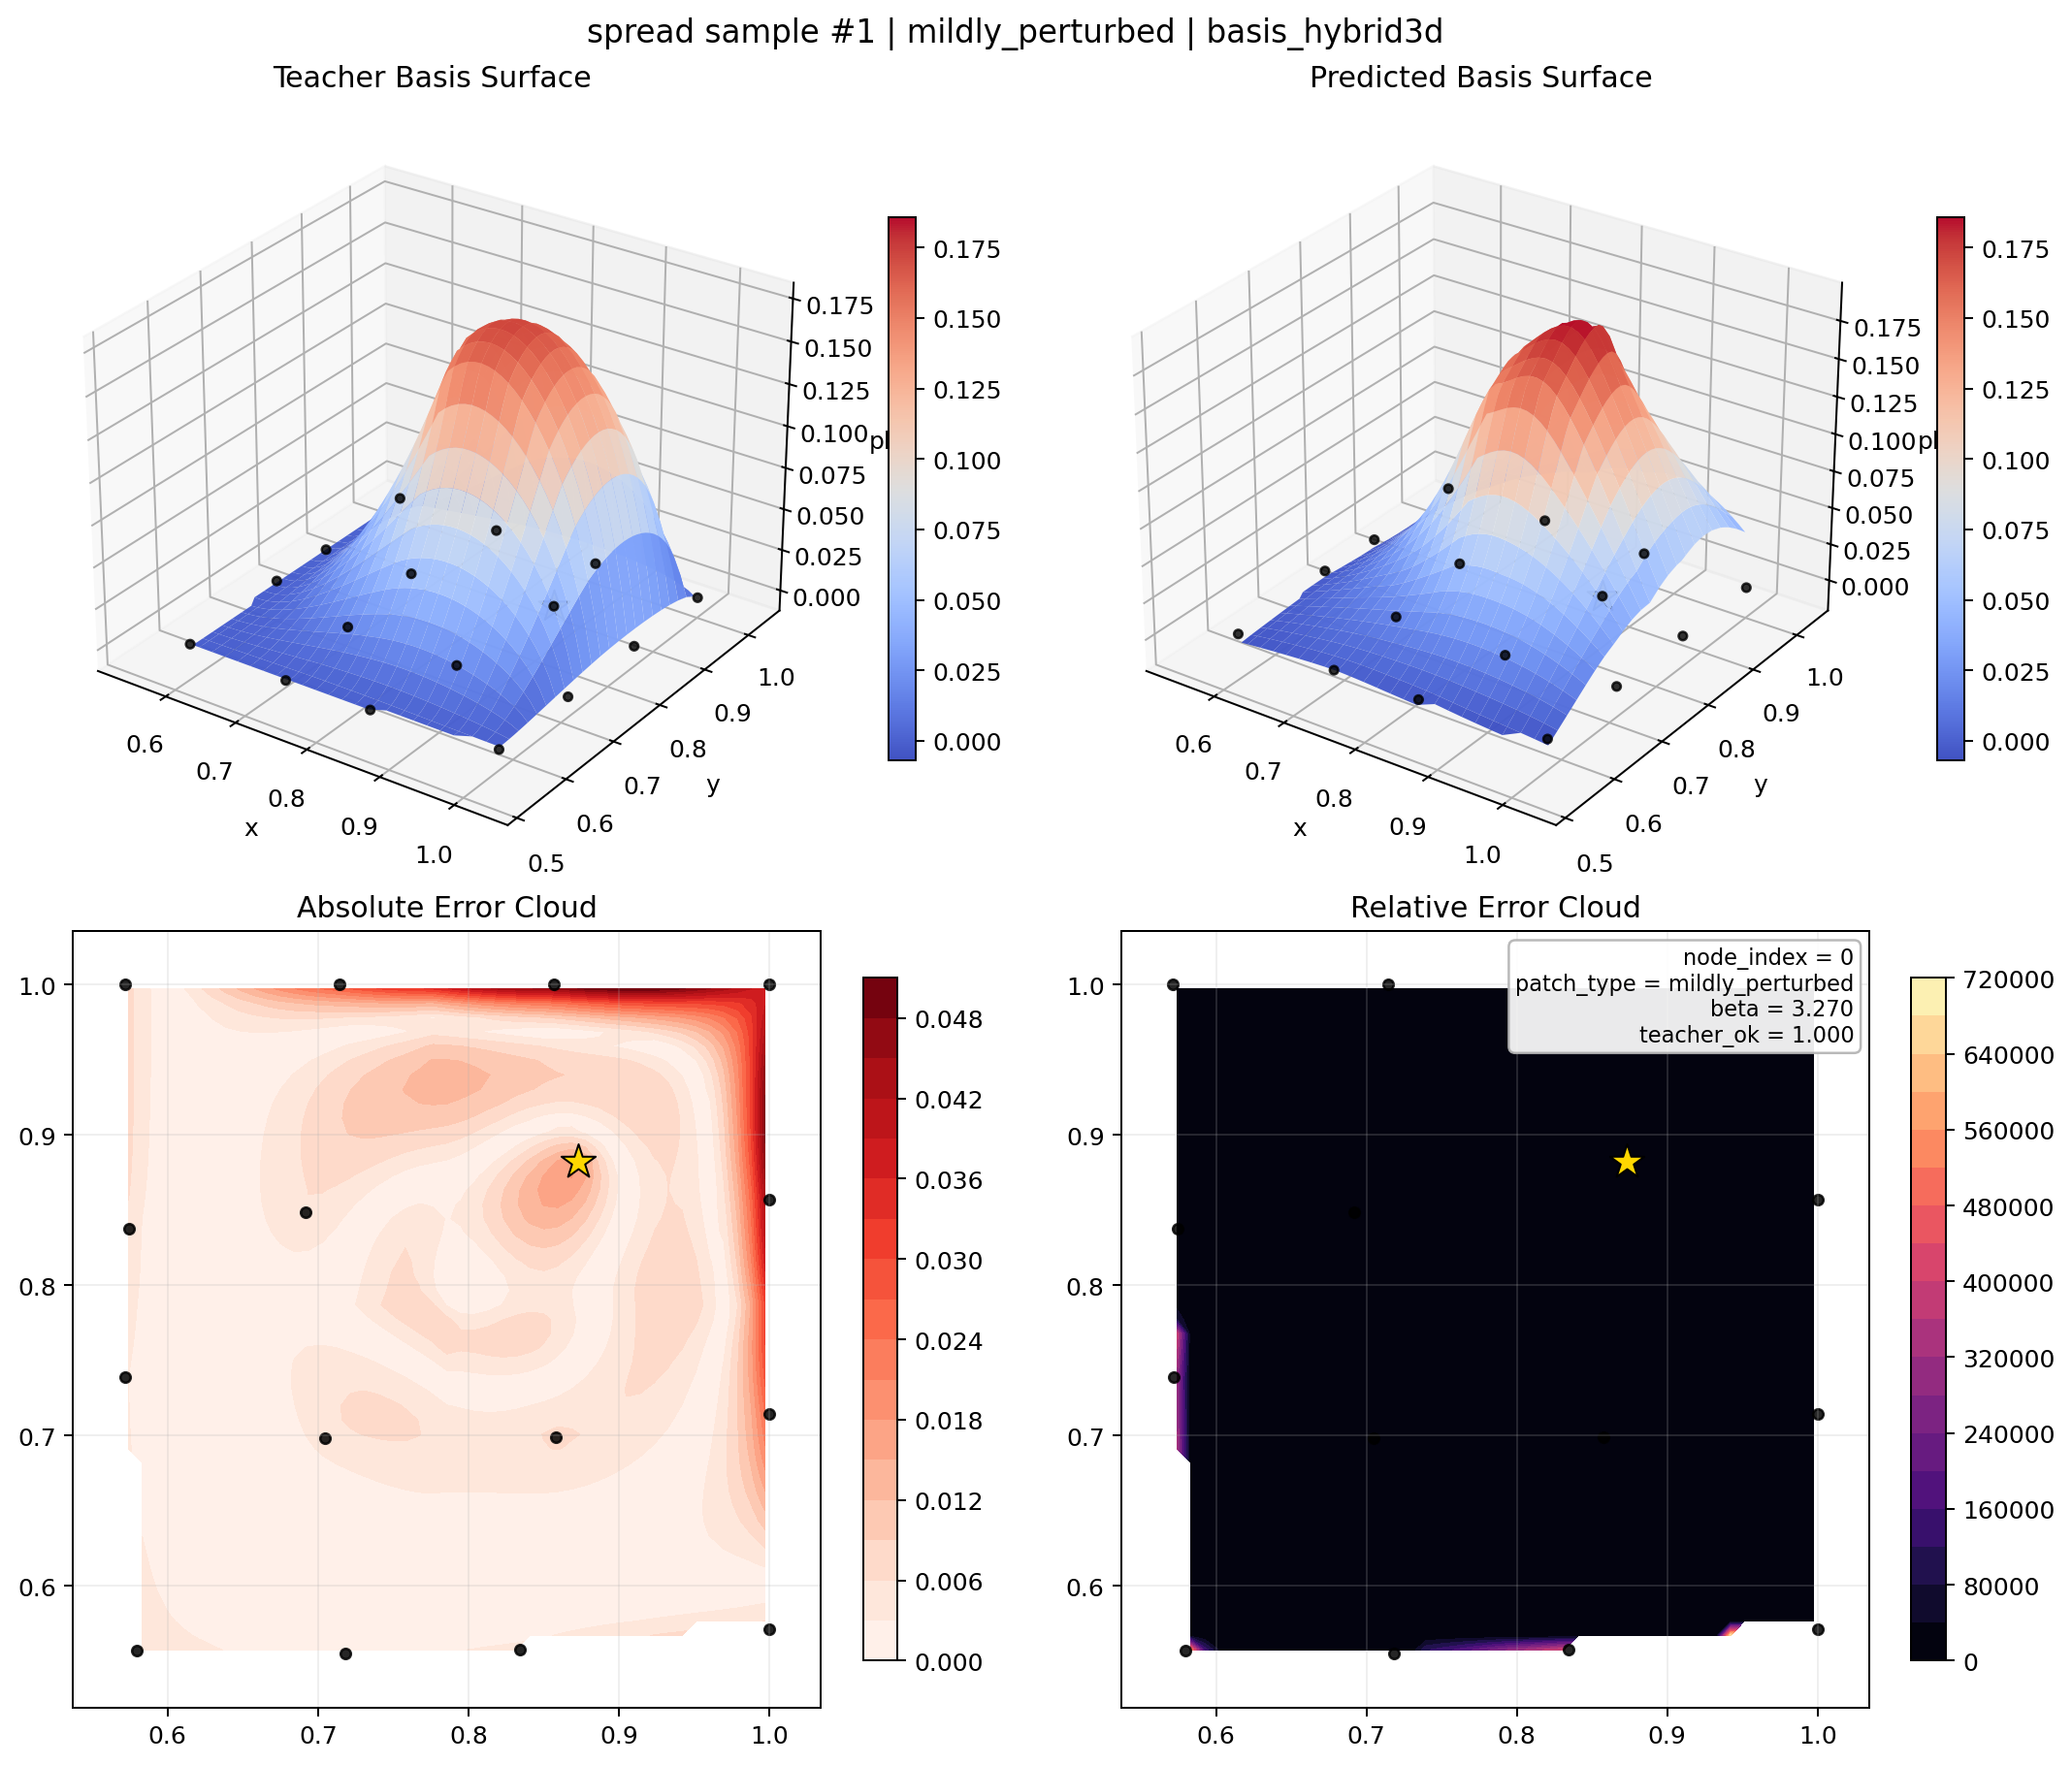
\includegraphics[width=\linewidth]{figures/basis_hybrid3d_normalcase.png}
  \end{columns}

  \vspace{0.5em}
  \begin{block}{代表性常规 patch}
    \begin{itemize}
      \item patch type：\texttt{mildly\_perturbed}，$\beta = 3.27$
      \item relative L2：$0.0141$，global $L_\infty$：$0.0026$
      \item 在常规工况下，teacher 与 prediction 基本重合
    \end{itemize}
  \end{block}
\end{frame}

\begin{frame}{常规验证样例}
  \begin{columns}[T,onlytextwidth]
    \column{0.48\textwidth}
      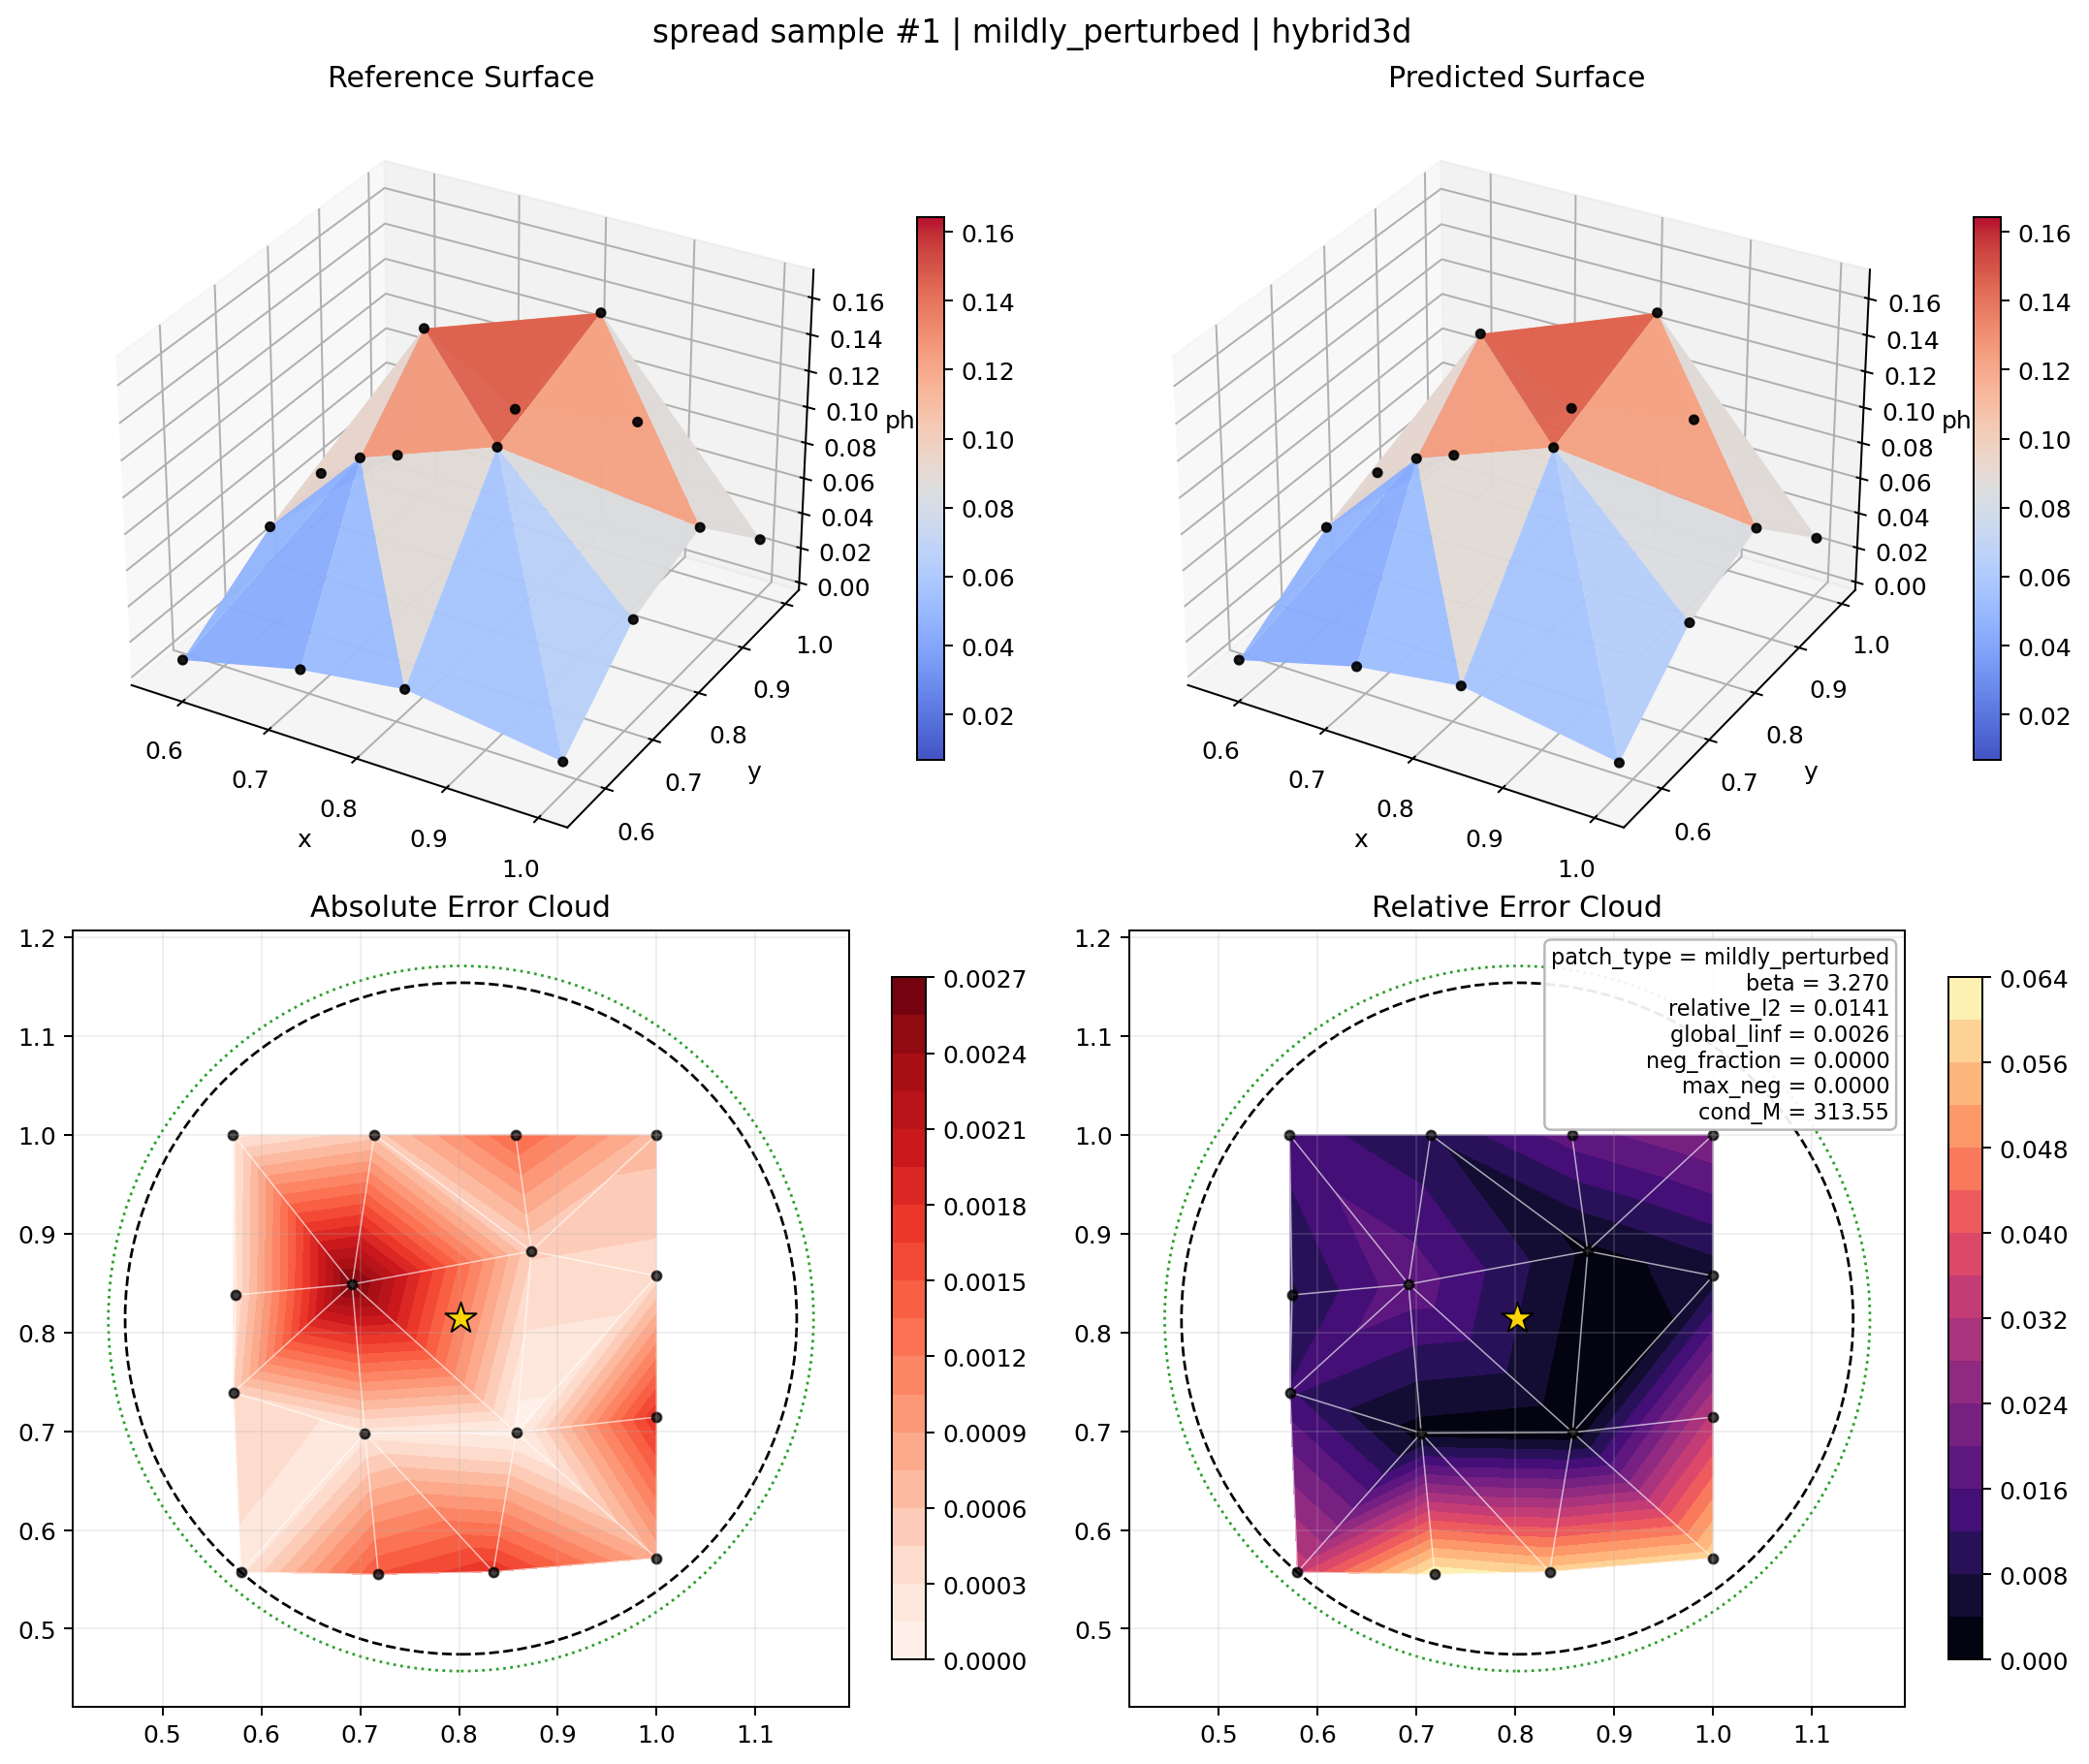
\includegraphics[width=\linewidth]{figures/spread_hybrid3d_normalcase.png}

      \vspace{0.4em}
      \small
      \textbf{样例 A：常规 mildly perturbed patch}\\
      relative L2 $= 0.0141$，global $L_\infty = 0.0026$

    \column{0.48\textwidth}
      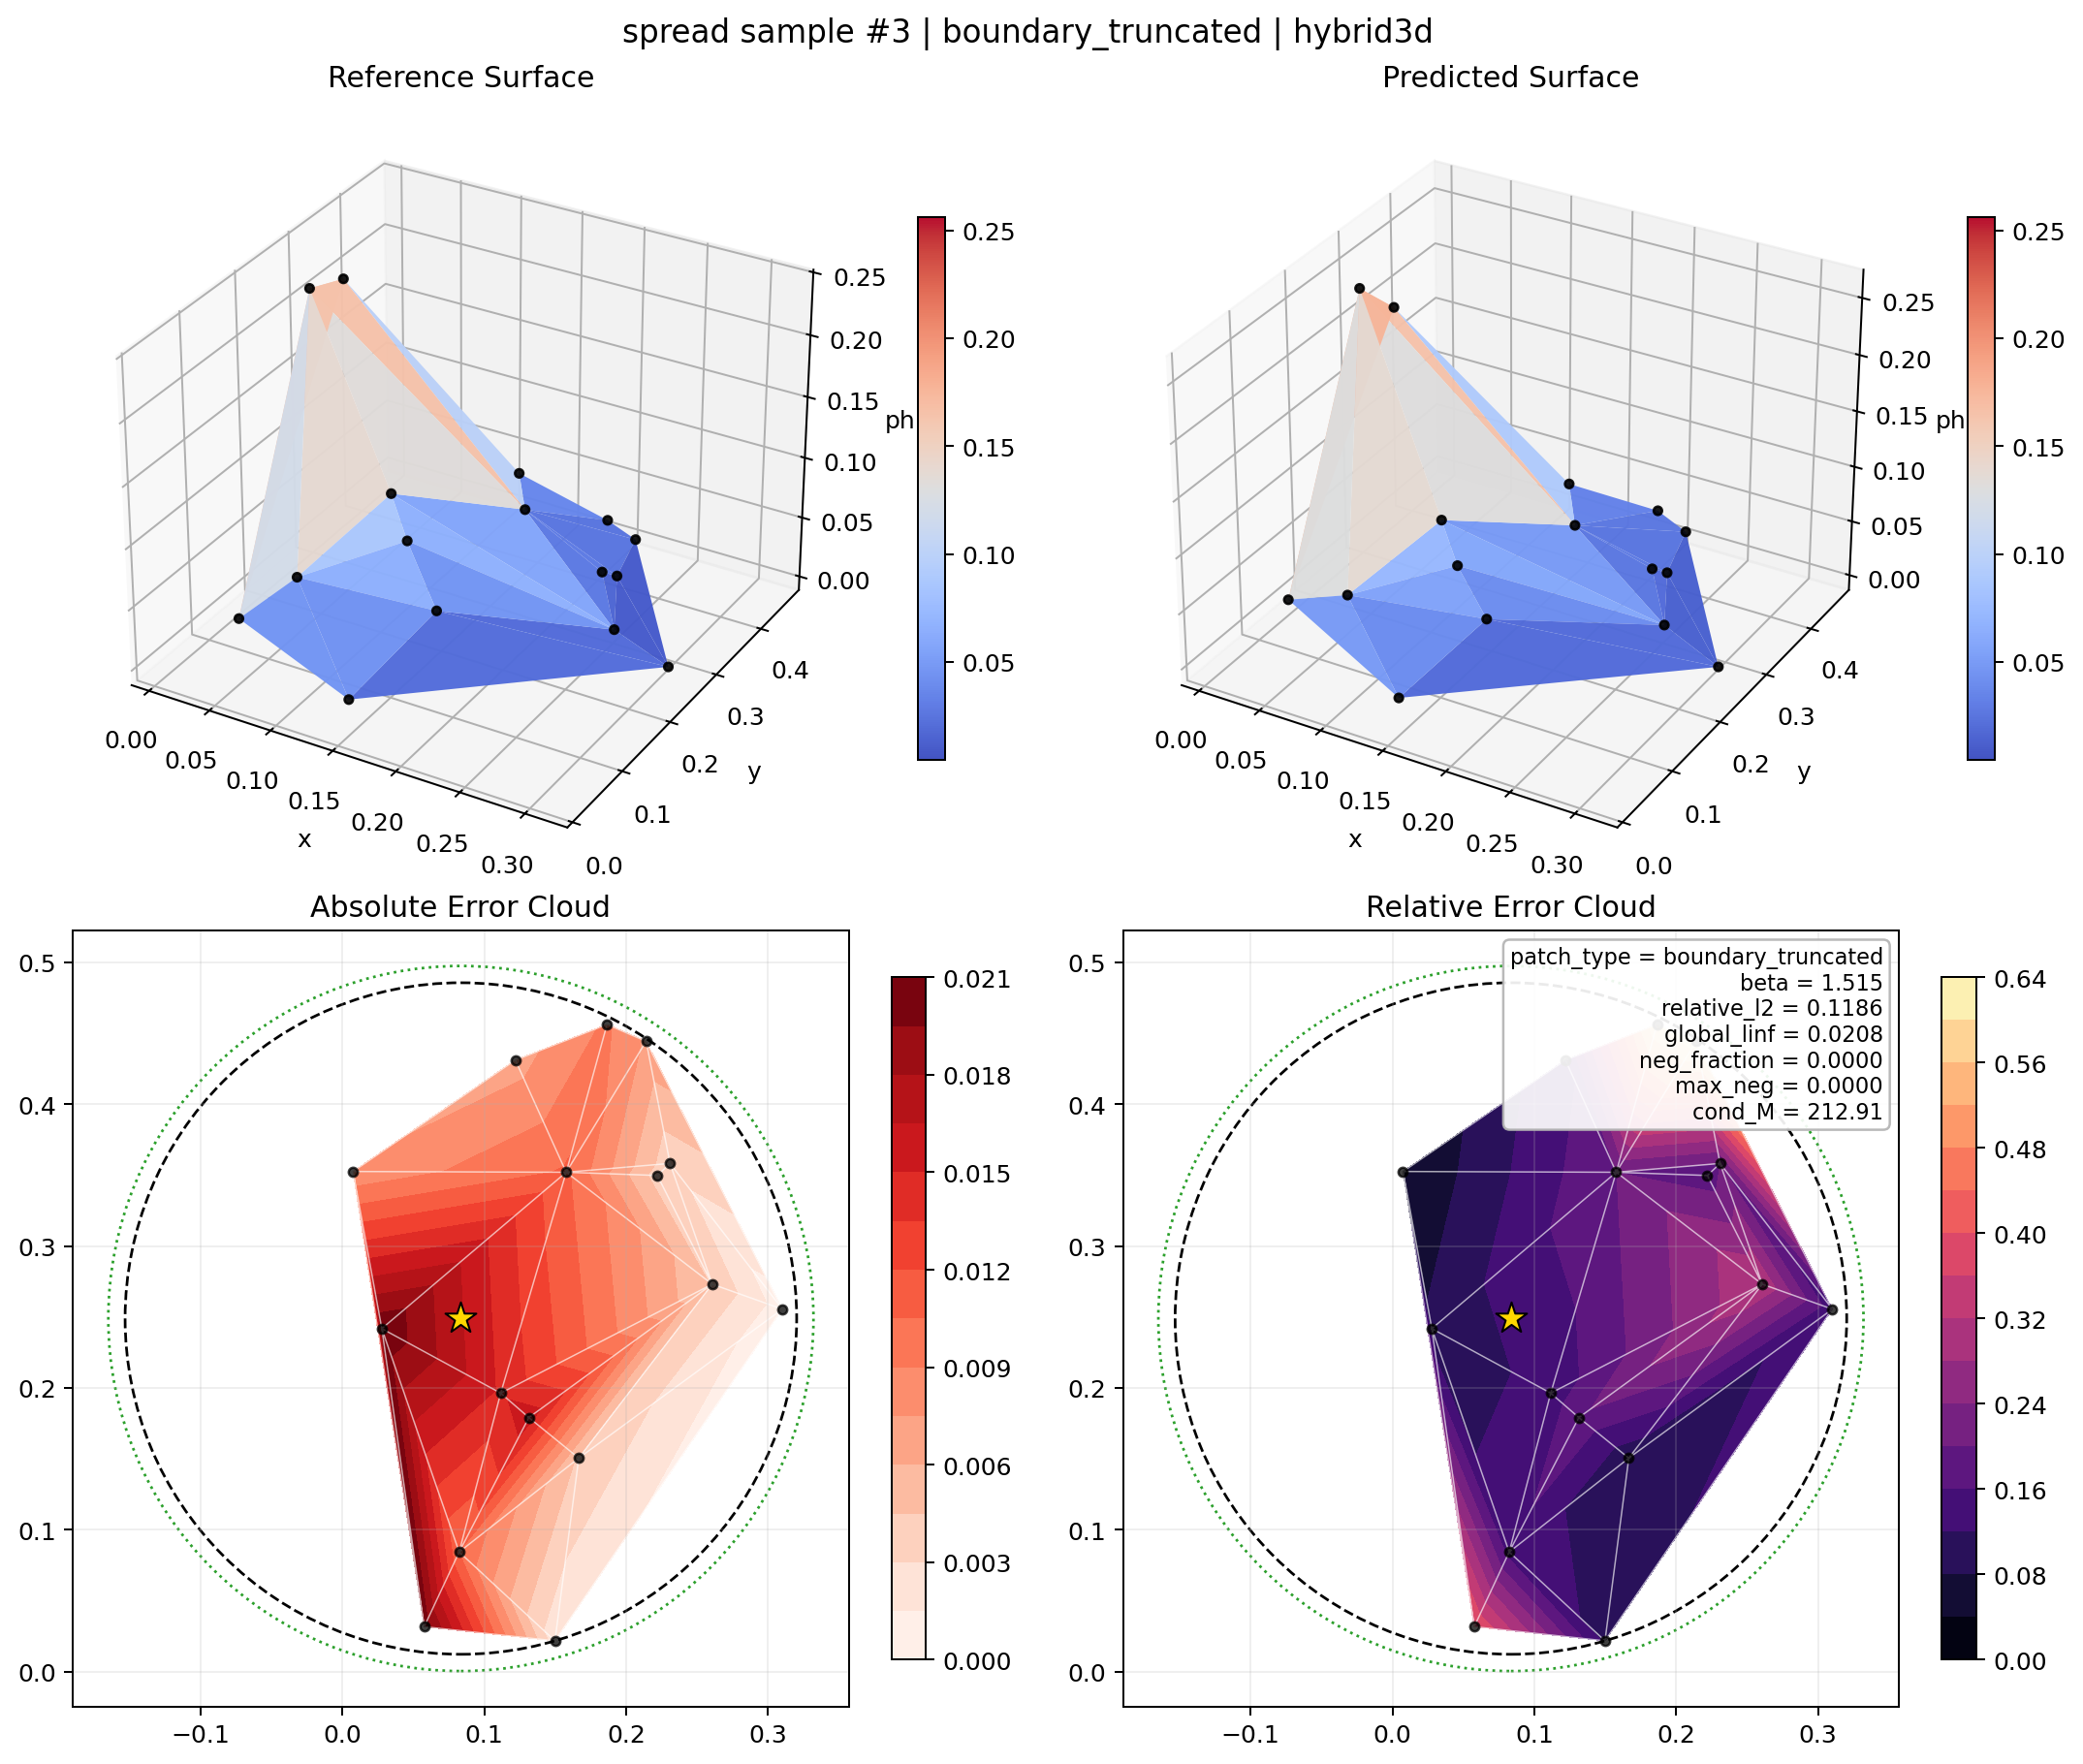
\includegraphics[width=\linewidth]{figures/spread_hybrid3d_regularcase.png}

      \vspace{0.4em}
      \small
      \textbf{样例 B：常规 boundary-truncated patch}\\
      relative L2 $= 0.1186$，整体仍然稳定
  \end{columns}

  \vspace{0.5em}
  \begin{block}{为什么要保留这些常规样例}
    \begin{itemize}
      \item 说明模型并不是只在最难样例或最坏样例上才有故事可讲。
      \item 常规 patch 可以验证 prediction 与 max-ent teacher 的接近程度。
      \item 常规截断 patch 则说明误差云图是局部集中的，而不是整体崩掉。
    \end{itemize}
  \end{block}
\end{frame}

\begin{frame}{代表性难例}
  \begin{columns}[T,onlytextwidth]
    \column{0.60\textwidth}
      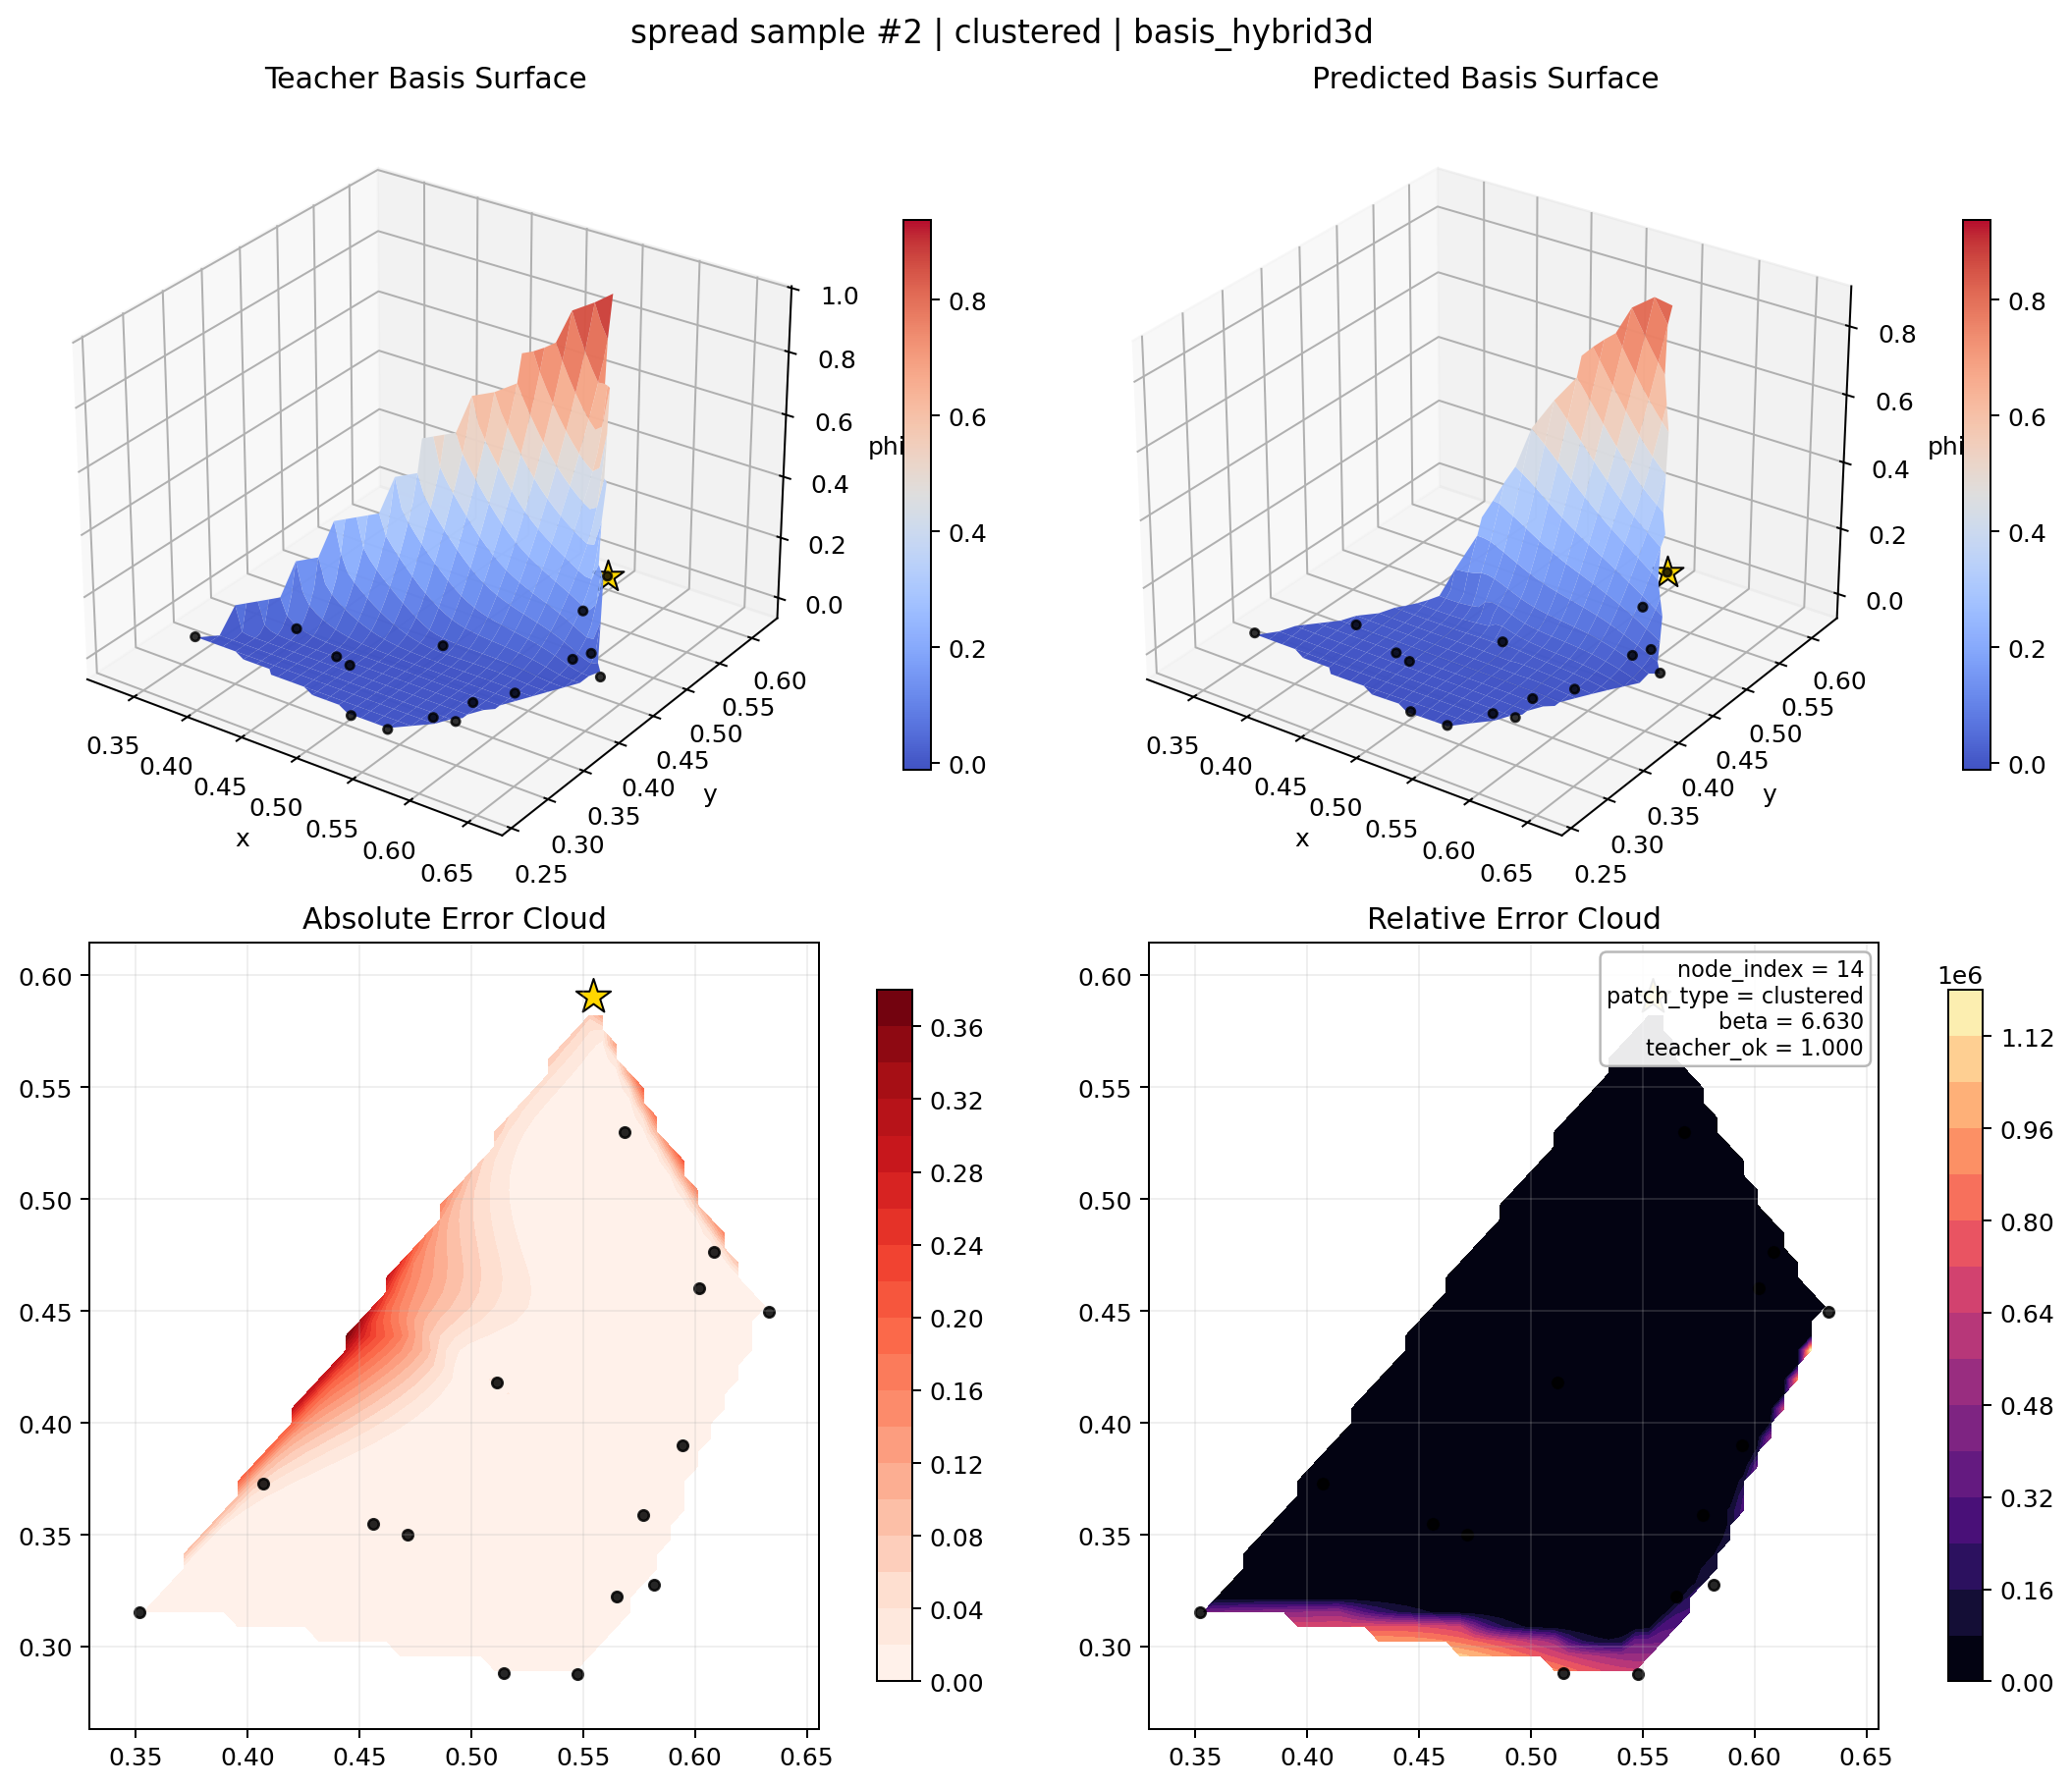
\includegraphics[width=\linewidth]{figures/basis_hybrid3d_hardcase.png}

    \column{0.36\textwidth}
      \begin{block}{观察到的现象}
        \begin{itemize}
          \item clustered / truncated patch 仍是当前最难的工况
          \item 难例中依然能看到局部误差集中
          \item 相比逐点误差，结构性指标要稳定得多
        \end{itemize}
      \end{block}

      \begin{alertblock}{Relative error 可视化}
        当前展示的 relative-error cloud 使用
        \[
        \frac{|\phi - \phi^{\mathrm{ref}}|}{\max(|\phi^{\mathrm{ref}}|,\varepsilon)}
        \]
        再配合 floor masking 与 clipping，因此接近 0 的区域不会再在图上爆炸。
      \end{alertblock}
  \end{columns}
\end{frame}

\begin{frame}{下一步}
  \begin{columns}[T,onlytextwidth]
    \column{0.49\textwidth}
      \begin{block}{方法侧}
        \begin{itemize}
          \item 继续检查 teacher prior 与 head locality 的一致性
          \item 做 head ablation，单独识别 B4 的贡献
          \item 构建 OOD patch 与 OOD-$\beta$ 评估
        \end{itemize}
      \end{block}

    \column{0.49\textwidth}
      \begin{block}{工程侧}
        \begin{itemize}
          \item 保持产物与图像入口的精简默认路径
          \item 继续提升 production run 的 GPU 利用率
          \item 把论文、PPT 与实验资产连成稳定工作流
        \end{itemize}
      \end{block}
  \end{columns}
\end{frame}

\begin{frame}[standout]
  谢谢
\end{frame}

\end{document}
